%
\documentclass[%
 reprint,
 amsmath,amssymb,
 aps,
]{revtex4-1}

\usepackage{graphicx}% Include figure files
\usepackage{dcolumn}% Align table columns on decimal point
\usepackage{bm}% bold math


\begin{document}


\title{ APRENDIZAJE SUPERVISADO}
\author{Damian Mamani, David Reynaldo
\and Jhony José Mamani Limache \and nombre  \and nombre }
		
\affiliation{%
 Universidad Privada de Tacna \textbackslash Facultad de Ingenieria \textbackslash Escuela Profesional de Ingenieria de Sistemas
}%

\begin{abstract}
\begin{center}
\textbf{Resumen}
\end{center}
completar
\\

\begin{center}
\textbf{Abstract}
\end{center}
completar
\\
\end{abstract}



\maketitle

%\tableofcontents

\section {Introducción}\label{sec:1}
La primera modalidad de aprendizaje que tiene el machine learning es la de aprendizaje supervisado. Usándola, se entrena al algoritmo otorgándole las preguntas, denominadas características, y las respuestas, denominadas etiquetas. Esto se hace con la finalidad de que el algoritmo las combine y pueda hacer predicciones.\\\\
Según se comentó en el primer artículo de esta serie, la clasificación es una subcategoría del aprendizaje supervisado en la que el objetivo es predecir las etiquetas de clase categóricas (discreta, valores no ordenados, pertenencia a grupo) de las nuevas instancias, basándonos en observaciones pasadas.\\
Esquema general de un modelo de aprendizaje supervisado
\begin{center}
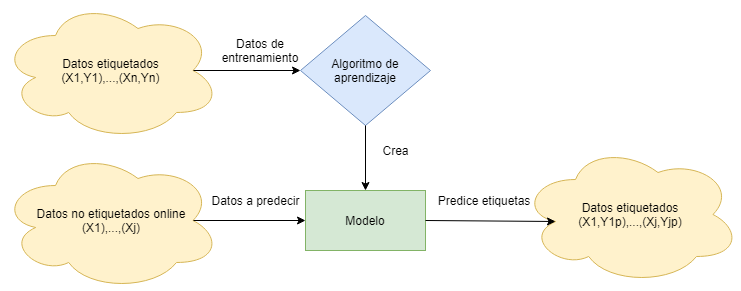
\includegraphics[width=7cm]{./Imagenes/esquemageneraldelmodelosupervisado}
\end{center}
 
Existen, a su vez, dos tipos de aprendizaje supervisado:\\
 \textbf{Regresión : }tiene como resultado un número específico. Si las etiquetas suelen ser un valor numérico, mediante las variables de las características, se pueden obtener dígitos como dato resultante.\\
 
 
\begin{center}
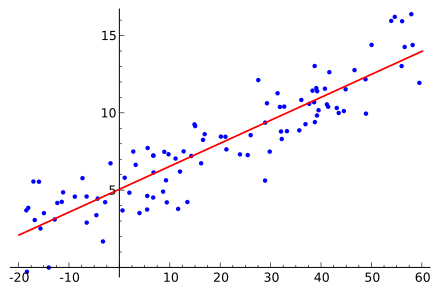
\includegraphics[width=7cm]{./Imagenes/regresion}
\end{center}
 
 \textbf{Clasificación : }en este tipo, el algoritmo encuentra diferentes patrones y tiene por objetivo clasificar los elementos en diferentes grupos.\\
 
 \begin{center}
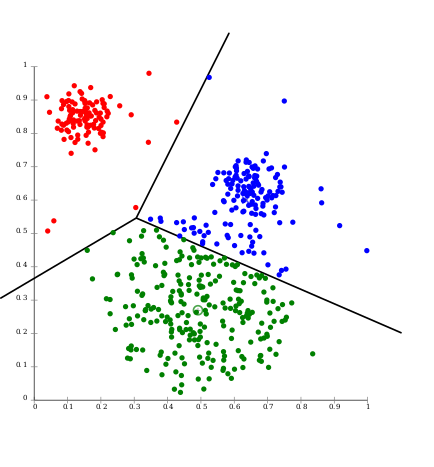
\includegraphics[width=7cm]{./Imagenes/clasificacion}
\end{center}

El algoritmo no está en capacidad de determinar a qué grupo pertenece un valor o cuál es el resultado de una operación. Solamente logra relacionar características con etiquetas y así obtener un resultado.\\\\

Hay dos tipos principales de clasificaciones:\\

 \textbf{Clasificación Binaria :} Es un tipo de clasificación en el que tan solo se pueden asignar dos clases diferentes (0 o 1). El ejemplo típico es la detección de email spam, en la que cada email es: spam → en cuyo caso será etiquetado con un 1 ; o no lo es → etiquetado con un 0.\\\\
  \textbf{Clasificación Multi-clase :}Se pueden asignar múltiples categorías a las observaciones. Como el reconocimiento de caracteres de escritura manual de números (en el que las clases van de 0 a 9).

 
%-----------------------------------------------------------------
\section{Objetivos}\label{sec:2}
\subsection{General:}
los algoritmos trabajan con datos “etiquetados” (labeled data), intentado encontrar una función que, dadas las variables de entrada (input data), les asigne la etiqueta de salida adecuada. El algoritmo se entrena con un “histórico” de datos y así “aprende” a asignar la etiqueta de salida adecuada a un nuevo valor, es decir, predice el valor da salida.
\subsection{Específicos:}
El aprendizaje supervisado se llama así porque el desarrollador actúa como una guía para enseñar al algoritmo las conclusiones a las que debe llegar, es decir la salida del algoritmo ya es conocida. Es similar a la forma en que un niño podría aprender de un maestro.
 \begin{center}
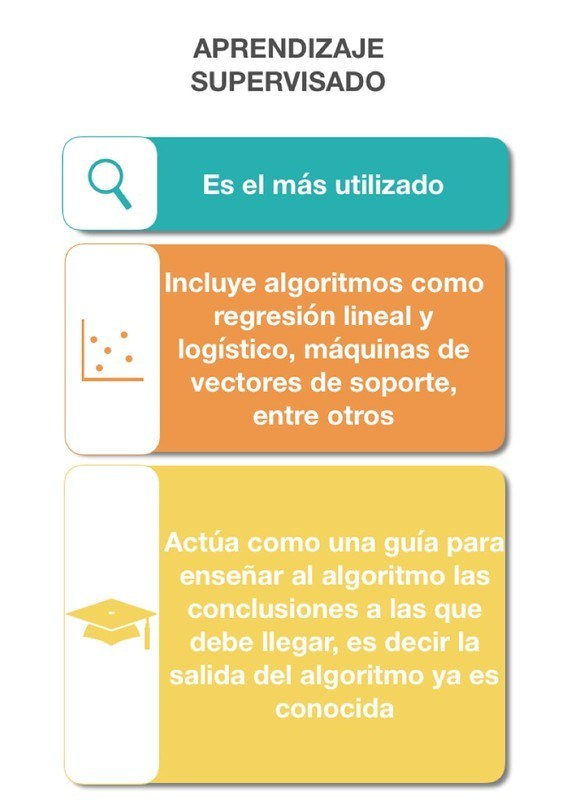
\includegraphics[width=5cm]{./Imagenes/objetivoprincipal}
\end{center}


%-----------------------------------------------------------------
\section {Marco Teórico}

\subsection{¿Que es aprendizaje supervisado?}	

%-------------------------------------------------
\subsection{Algoritmos que se usan en aprendizaje supervisado}	

%-------------------------------------------------

\subsection{Aprendizaje supervisado por regresion y por clasificacion}

%-------------------------------------------------
\subsection{Ventajas,Desventajas e importancia}

  \textbf{VENTAJAS :}\\ • Es posible dar un algoritmo general para su aplicación. Es decir, se trata de un mecanismo muy bien definido, que no depende apenas del tipo de problema de clasificación al que nos enfrentamos. \\
  • Tenemos cierta seguridad sobre lo que puede hacer el clasificador y lo que no puede hacer.\\ • Durante el entrenamiento podemos medir el grado de acierto del clasificador y podemos detener el entrenamiento cuando lo consideremos aceptable.\\
  
    \textbf{DESVENTAJAS :} \\• Tenemos que el proceso de entrenamiento suele ser lento y no es infalible, se depende bastante de la elección de los casos de entrenamiento para que el clasificador sea capaz de generalizar lo suficiente.\\ • Es preciso un trabajo previo de clasificación manual de los casos que se usarán para el entrenamiento, que pueden ser muchos miles en un problema de cierta complejidad.\\
    
    \textbf{IMPORTANCIA :} \\
    El aprendizaje supervisado proporciona una ruta directa para convertir datos en información real y procesable. Al utilizar los datos como un recurso, les permite a las organizaciones comprender y prevenir los resultados no deseados o impulsar los resultados deseados para lo que sea que estén tratando de predecir.\\
    Por ejemplo, pueden decirle a una empresa que los clientes presentan un alto riesgo de agitación, la compañía puede llegar a ese cliente en particular con comunicaciones dirigidas y ofertas promocionales, lo que reduce su predisposición al abandono.\\
    Este aprendizaje es uno de los motores más potentes que permite que los sistemas de inteligencia artificial tomen decisiones empresariales de forma más rápida y precisa que los humanos.

 \begin{center}
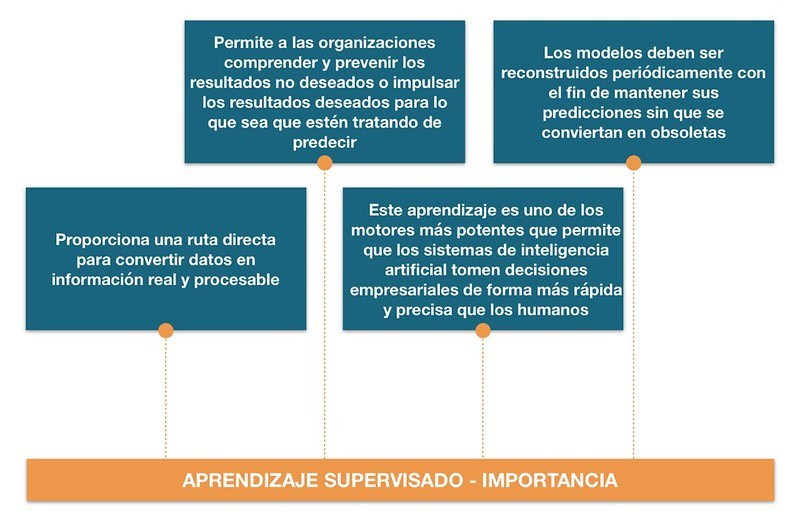
\includegraphics[width=7cm]{./Imagenes/importancia}
\end{center}

%-------------------------------------------------


\section{Ejemplo}

%-----------------------------------------------------------------
\section{Análisis}

\begin{itemize}
\item
completar

\end{itemize}
%-----------------------------------------------------------------
\section{Conclusiones}

\begin{itemize}
\item 
completar

\end{itemize}

\newpage
% Bibliografia.
%-----------------------------------------------------------------

\begin{thebibliography}{99}
http://machinelearningparatodos.com/tipos-de-aprendizaje-automatico/\\
https://www.toptal.com/machine-learning/explorando-algoritmos-de-aprendizaje-automatico-supervisado\\
https://medium.com/datos-y-ciencia/aprendizaje-supervisado-introducci%C3%B3n-a-la-clasificaci%C3%B3n-y-principales-algoritmos-dadee99c9407\\
https://medium.com/@juanzambrano/aprendizaje-supervisado-o-no-supervisado-39ccf1fd6e7b\\
http://ligdigonzalez.com/todo-sobre-aprendizaje-supervisado-en-machine-learning/\\
http://ligdigonzalez.com/diferencia-entre-aprendizaje-supervisado-y-no-supervisado/\\
https://empresas.blogthinkbig.com/que-algoritmo-elegir-en-ml-aprendizaje/\\

\bibitem{Cd94} Autor, \emph{Título}, Revista/Editor, (año)

\end{thebibliography}


\end{document}
